\chapter{Практическая часть}
\label{cha:ch_2}

В рамках ВКР была реализована
библиотека hpfw (\href{https://github.com/kisasexypantera94/hpfw}{\color{blue} ссылка} на Github).
С использованием инструментов библиотеки была решена задача идентификации музыкальных
произведений по фрагментам концертных исполнений. Для этой же
задачи написан Telegram-бот (\href{https://t.me/hpfw_bot}{\color{blue} ссылка} на бота).

\section{Технологии}
В библиотеке hpfw используются:
\begin{itemize}
    \item C++17
    \item essentia -- для вычисления спектрограмм
    \item Eigen3 -- для линейной алгебры
    \item cpp-taskflow -- для распараллеливания индексации
\end{itemize}

Для библиотеки также написан Python-клиент.

\section{Архитектура библиотеки}
В центре библиотеки два класса -- $Collector$ (коллектор) и $HashprintHandle$ (хеншпринт-хендл).
Эти классы связаны паттерном <<Стратегия>>. Хендлы предоставляют инструменты (функции) для вычисления
хешпринтов. Коллекторы используют эти инструменты по своему усмотрению и занимаются непосредственно
вычислением хешпринтов. Благодаря такой структуре, можно будет легко тестировать различные способы
распараллеливания индексации.

\section{Клиент}
Пока что не очень ясно, где стоит проводить черту между библиотекой и клиентом. На данный момент
клиент использует только класс $Collector$.

\section{Telegram-бот}
Пример работы:
\begin{figure}[H]
    \centering
    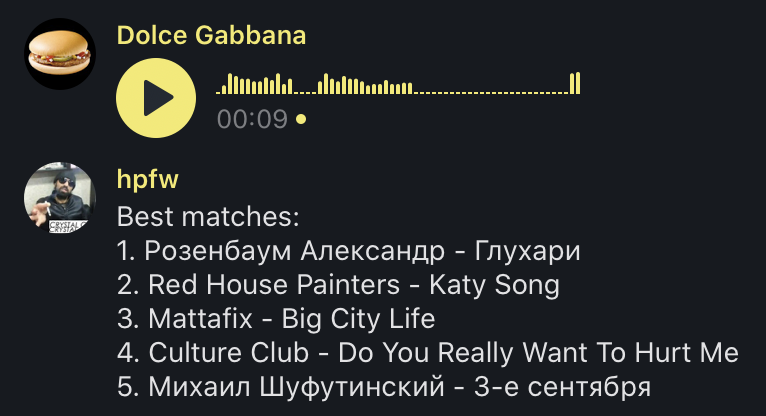
\includegraphics[scale=0.6]{inc/img/tgbot.png}
    \caption{}
\end{figure}

\section{Результаты}
Замеры проводились на Intel i5-6360U (4) @ 2.00GHz, 8GB RAM
\begin{itemize}
    \item На индексацию одного трека уходит в среднем 5.7 секунд
    \item На полный поиск отрывка по базе из 167 треков (без индекса) уходит 4 миллисекунды
    \item Точность поиска 216 9-секундных отрывков по базе из 167 треков -- 0.78.
    \item Одна спектрограмма занимает около 10 МБ (правда, их не всегда нужно хранить)
\end{itemize}

Стоит отметить, что поиск осуществлялся без знания исполнителя, то есть это оценка в худшем случае.